% !TEX root = ../main.tex

%----------------------------------------------------------------------
\subsection{Defect-aware periodic graph construction}\label{sec:graph}
%----------------------------------------------------------------------

Each defect supercell is represented as a graph $\mathcal{G} = (\mathcal{V},
\mathcal{E})$ where nodes correspond to atoms and edges to interatomic
interactions.

\paragraph{Minimum-image neighbor list.}
For a 2D monolayer with lattice vectors $\mathbf{L} = [\mathbf{l}_1,
\mathbf{l}_2, \mathbf{l}_3]$ and periodic boundary conditions (PBC), the
neighbor set of atom $i$ is
\begin{equation}\label{eq:neighbors}
  \mathcal{N}(i) = \bigl\{(j, \mathbf{n}) \in V \times \mathbb{Z}^3
    \;\big|\; \|\mathbf{r}_j + \mathbf{L}\mathbf{n} - \mathbf{r}_i\|
    < r_\mathrm{cut},\; \mathbf{n}\text{ minimizes distance}\bigr\},
\end{equation}
with $r_\mathrm{cut} = 5.0$\,\AA{}.

\paragraph{Node features.}
Each atom $i$ is described by a 9-dimensional physicochemical feature vector
$\mathbf{x}_i$ comprising group, period, Pauling electronegativity, covalent
radius, van der Waals radius, number of valence electrons, first ionization
energy, electron affinity, and atomic mass.
All features are $z$-score normalized across the periodic table.

\paragraph{Defect-site embedding.}
A binary indicator $\delta_i \in \{0, 1\}$ marks whether atom $i$ is the
dopant (substitutional defect) or resides at an interstitial/adsorbate site:
\begin{equation}\label{eq:defect_embed}
  \mathbf{h}_i^{(0)} = \mathbf{W}_\mathrm{emb}\,\mathbf{x}_i
    + \mathbf{e}_\mathrm{def}(\delta_i),
\end{equation}
where $\mathbf{e}_\mathrm{def}$ is a learned $\mathbb{R}^2 \to \mathbb{R}^d$
embedding.
This explicit marker injects the defect location into the initial
representation, guiding the attention mechanism to focus on the defect core
and its surroundings.

\paragraph{Edge features.}
Interatomic distances $d_{ij}$ are expanded via Gaussian radial basis
functions (RBF):
\begin{equation}
  e_{ij,k} = \exp\!\Bigl(-\frac{(d_{ij} - \mu_k)^2}{\sigma^2}\Bigr),
  \quad k = 1, \ldots, K,
\end{equation}
with $K = 32$ centers uniformly spaced in $[0, r_\mathrm{cut}]$.

\paragraph{Bond-angle triplets.}
For each center atom $i$ and neighbor pair $(j, k) \in \mathcal{N}(i)^2$, we
compute the bond angle $\theta_{jik}$ via the dot product of displacement
vectors.
Angles are expanded by a second RBF over $[0, \pi]$ and processed by an MLP,
encoding three-body correlations critical for distinguishing local bonding
geometries.

%----------------------------------------------------------------------
\subsection{DART architecture}\label{sec:arch}
%----------------------------------------------------------------------

\dart{} adopts a hierarchical design that decouples short-range chemical
bonding from long-range defect-induced perturbations
(Fig.~\ref{fig:architecture}).

\begin{figure*}[t]
\centering
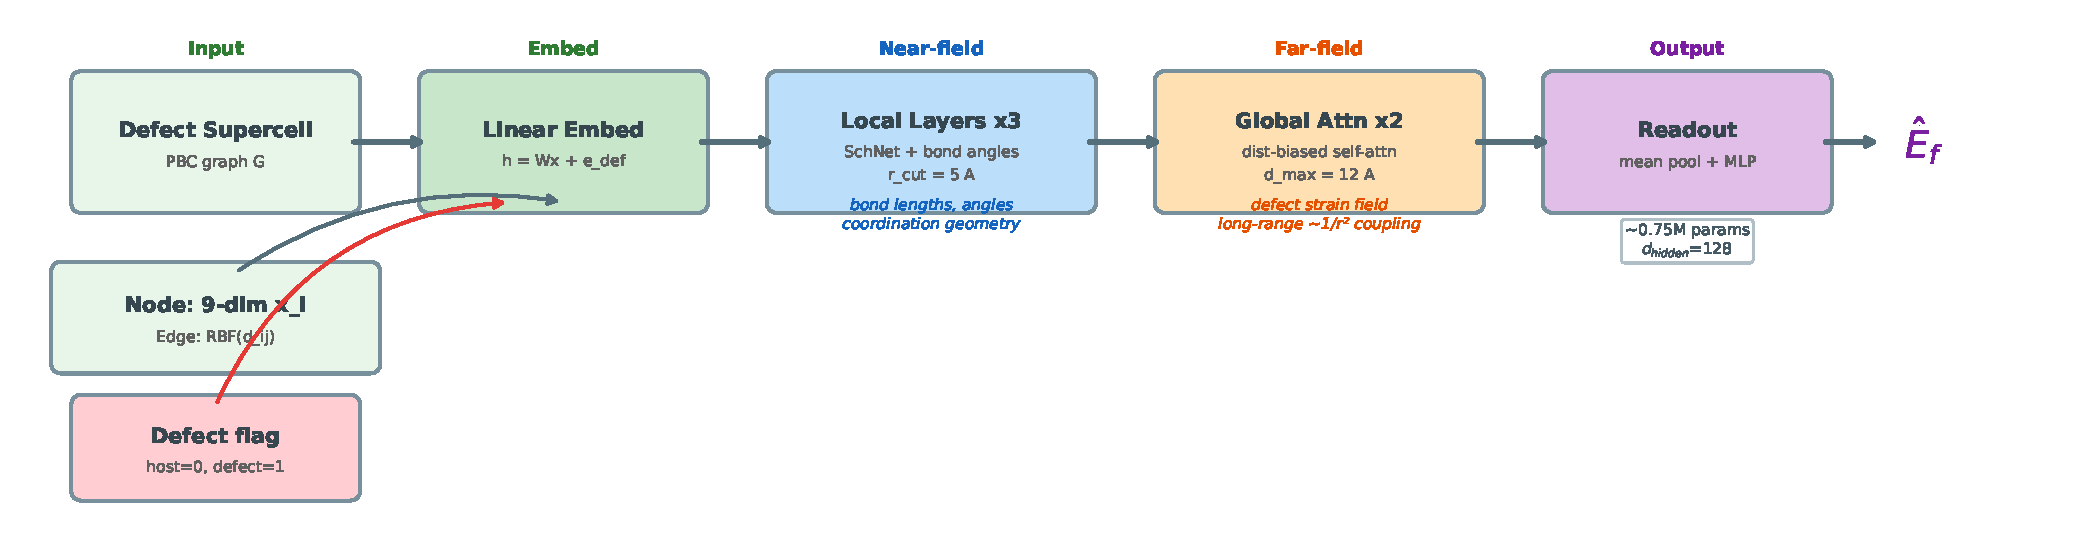
\includegraphics[width=\textwidth]{figures/architecture.pdf}
\caption{\dart{} architecture overview.
  Local interaction layers (blue) capture bond lengths, bond angles, and
  coordination within $r_\mathrm{cut} = 5$\,\AA{}.
  Global geometric self-attention layers (orange) model long-range
  defect-induced perturbations via distance-biased attention up to
  $d_\mathrm{max} = 12$\,\AA{}.
  An explicit defect-site embedding (red) injects the dopant location.}
\label{fig:architecture}
\end{figure*}

\subsubsection{Local interaction layers}

The first $L_\mathrm{loc} = 3$ layers operate on the sparse neighbor graph.
Each layer updates atom features via continuous-filter convolution gated by
distance, with additive three-body angle modulation:
\begin{equation}\label{eq:local}
  \mathbf{h}_i^{(l+1)} = \mathbf{h}_i^{(l)}
    + \sigma\!\Biggl(
      \sum_{j \in \mathcal{N}(i)} \boldsymbol{\phi}(d_{ij})
        \odot \mathbf{W}\mathbf{h}_j^{(l)}
      + \!\!\sum_{(j,k) \in \mathcal{T}(i)}\!\!
        f_\mathrm{trip}(\mathbf{h}_i^{(l)}, \theta_{jik})
    \Biggr),
\end{equation}
where $\boldsymbol{\phi}$ is a two-layer MLP over the RBF-expanded distance,
$\mathcal{T}(i)$ denotes the triplet set of atom $i$ (capped at 32),
$f_\mathrm{trip}$ is an MLP over concatenated atom features and
angle RBF, and $\sigma$ is the SiLU activation.
These layers precisely encode the near-field chemical environment:
bond lengths, bond angles, and coordination geometry within the first
neighbor shell.

\subsubsection{Global geometric self-attention layers}

The subsequent $L_\mathrm{glob} = 2$ layers employ full multi-head
self-attention over all atoms in the supercell, with a learnable distance
bias that injects periodic geometry:
\begin{equation}\label{eq:global_attn}
  \mathrm{Attn}(Q, K, V)
    = \mathrm{softmax}\!\left(
        \frac{QK^\top}{\sqrt{d_k}}
        + \phi_\mathrm{bias}\!\bigl(d_{ij}^{\mathrm{PBC}}\bigr)
      \right) V,
\end{equation}
where $d_{ij}^{\mathrm{PBC}} = \min_{\mathbf{n} \in \mathbb{Z}^3}
\|\mathbf{r}_i - \mathbf{r}_j + \mathbf{L}\mathbf{n}\|$ is the
minimum-image distance (computed up to $d_\mathrm{max} = 12$\,\AA{}),
and $\phi_\mathrm{bias}: \mathbb{R} \to \mathbb{R}^{N_\mathrm{heads}}$ maps
RBF-expanded distances through an MLP to per-head attention biases.

\paragraph{Physical interpretation.}
Following the ``neural potential summation'' framework of
Taniai~\textit{et al.}~\cite{crystalformer2024}, the distance bias
$\phi_\mathrm{bias}(d_{ij}^{\mathrm{PBC}})$ can be interpreted as a
\emph{learnable interatomic potential} that modulates information flow:
even atoms without topological edges (beyond $r_\mathrm{cut}$) can exchange
information if the learned potential assigns non-negligible coupling at their
separation.
%
Concretely, the Gaussian RBF expansion
$e_{ij,k} = \exp(-(d-\mu_k)^2/\sigma^2)$ that feeds $\phi_\mathrm{bias}$
forms a localized basis in real space, analogous to how plane-wave
expansions $e^{i\mathbf{G}\cdot\mathbf{r}}$ form a basis in reciprocal
space.
By learning linear combinations of these Gaussians, the model implicitly
constructs a smooth, distance-dependent coupling function---effectively
performing a ``soft'' Fourier-like decomposition of the interatomic
interaction landscape.
%
This mechanism is particularly relevant for point defects in 2D, whose
strain fields and charge-density perturbations decay as
${\sim}1/r^2$~\cite{fang2025}, well beyond typical GNN cutoff radii.

The defect embedding $\mathbf{e}_\mathrm{def}$ ensures that the dopant atom
occupies a distinct region in the query space, naturally emerging as an
attention hub---a prediction confirmed by our interpretability analysis
(\S\ref{sec:interpret}).

\subsubsection{Readout}

Atom-level representations are aggregated by masked mean pooling and passed
through a two-layer MLP with LayerNorm to predict $\ef$:
\begin{equation}
  \hat{E}_\mathrm{f} = \mathrm{MLP}\!\left(
    \frac{\sum_{i} m_i \,\mathbf{h}_i^{(L)}}
         {\sum_{i} m_i}
  \right),
\end{equation}
where $m_i$ is the atom mask.
The total parameter count is ${\approx}0.75$\,M for
$d_\mathrm{hidden} = 128$.

%----------------------------------------------------------------------
\subsection{Training pipeline}\label{sec:training}
%----------------------------------------------------------------------

We employ a systematic training recipe optimized for the data-limited regime
(${\sim}8.5$\,k training samples):

\begin{itemize}
  \item \textbf{MAE (L1) loss.}
    The $\ef$ distribution has a long tail (range $[-15, +18]$\eV{}),
    making $\ell_1$ robust to outliers and directly aligned with the
    evaluation metric.

  \item \textbf{Cosine annealing with linear warmup.}
    A 10-epoch linear warmup from $10^{-7}$ to $5\times10^{-4}$ stabilizes
    early optimization under the non-smooth $\ell_1$ gradient, followed by
    cosine decay to $10^{-6}$ over 150 epochs.

  \item \textbf{Stochastic Weight Averaging (SWA).}
    From epoch 120, model weights are averaged every epoch, promoting
    convergence to flatter minima with better generalization
    properties~\cite{swa2018}.

  \item \textbf{ct-UAE pretrained atomic embeddings.}
    128-dimensional universal atomic embeddings from a CrystalTransformer
    pretrained on Materials Project~\cite{ctuae2025} are concatenated to
    $\mathbf{x}_i$ before the embedding layer, injecting transferable
    chemical priors.

  \item \textbf{Label noise regularization.}
    Gaussian noise ($\sigma = 0.03$\eV{}) is added to training targets,
    simulating DFT numerical uncertainty and preventing overfitting to
    exact labels.

  \item \textbf{Online data augmentation.}
    Random in-plane rotations, coordinate perturbations
    ($\sigma_r \in [0.01, 0.05]$\,\AA{}), and biaxial strain
    ($\leq 2\%$) are applied on-the-fly, enforcing rotational and
    translational invariance.
\end{itemize}

\paragraph{Multi-source data fusion.}
A key challenge in training on small materials databases is that the model
never encounters enough structural diversity to learn robust atomic
representations.
We address this by jointly training on four databases with complementary
coverage:
(i)~IMP2D~\cite{imp2d2023} (10\,641 2D defect configurations, primary
target),
(ii)~JARVIS-2D (1\,105 pristine 2D formation energies),
(iii)~JARVIS-3D (4\,457 bulk formation energies), and
(iv)~a curated DFT-3D set (10\,987 bulk crystals from the Materials
Project), totaling ${\sim}27$\,k samples.
%
Because the four databases differ in dimensionality (2D vs.\ 3D),
defect content (impurity vs.\ pristine), and label semantics (defect
$\ef$ vs.\ bulk formation energy), a naive merge would degrade
performance.
We instead adopt a \emph{multi-head} architecture: the local and global
encoder layers are shared across all sources, but each source feeds into
its own independent two-layer readout MLP.
During training, batches are drawn from all sources with tunable
per-source sampling weights (IMP2D\,$=$\,1.0, JARVIS-2D\,$=$\,0.5,
JARVIS-3D\,$=$\,0.5, DFT-3D\,$=$\,0.1), and each sample's loss is
routed through its corresponding head.
This prevents label-space contamination while allowing the shared encoder
to learn transferable structural representations---particularly for
rare dopant elements that appear in auxiliary databases but have few
IMP2D entries.

%----------------------------------------------------------------------
\subsection{Ensemble and uncertainty quantification}\label{sec:uq_method}
%----------------------------------------------------------------------

We construct a pool of 29 models spanning six diversity axes: random seed
(5 values), loss function (MAE/Huber), architecture depth (shallow/deep),
embedding type ($\pm$ct-UAE), training epochs (100/150), and training data
(single-source/multi-source).
A greedy forward selection algorithm identifies the $k$-model subset
minimizing validation MAE; the optimal $k=7$ achieves 0.359\eV{}.

Prediction uncertainty is estimated as the standard deviation of ensemble
member predictions.
Post-hoc temperature scaling~\cite{guo2017} with parameter $\tau$ is
calibrated on the validation set to align the nominal and empirical coverage
of prediction intervals.

%----------------------------------------------------------------------
\subsection{Graduated Generalization Assessment}\label{sec:ood_method}
%----------------------------------------------------------------------

Random test splits overestimate real-world performance because chemically
similar configurations leak across partitions~\cite{li2025ood,omee2024}.
We propose a three-tier protocol with increasing extrapolation difficulty:

\begin{description}
  \item[Tier~0 (ID):]
    Standard 80/10/10 random split.
    Tests interpolation within the training distribution.

  \item[Tier~1 (Intra-family OOD):]
    Leave-one-host-out (LOHO) cross-validation over the seven G6-TMD
    hosts\footnote{MoS$_2$, MoSe$_2$, MoTe$_2$, WS$_2$, WSe$_2$,
    WTe$_2$, MoSSe.}:
    in each fold, \emph{all} configurations of one host are held out while
    the remaining six hosts (plus all non-G6 hosts) form the training set.
    This tests transfer to a chemically related but unseen host material.

  \item[Tier~2 (Compositional OOD):]
    G6$\times$3d block-out: all configurations pairing a G6 host with a
    3d-block dopant (Sc--Zn) are held out, testing matrix-completion
    generalization for unseen (host, dopant) combinations.
\end{description}
